 \subsection{Einführungsbeispiel}
Das zentrale Thema dieses Abschnitts sind Orthogonalprojektionen regulärer Polyeder auf Ebenen. Als Einstieg betrachten wir die Projektion eines Würfels auf eine Ebene im Raum. Der Würfel, auch \textbf{reguläres Hexaeder} genannt, siehe Abb. \ref{fig:einheitswürfel}, besitzt zahlreiche interessante Merkmale. Dazu gehören insbesondere seine Symmetrieeigenschaften, welche in Abschnitt \ref{sec:symmetrieeigenschaftwürfel} detailliert analysiert werden. Im Rahmen dieses Einführungsbeispiels fokussieren wir uns jedoch primär auf eine spezifische Eigenschaft der Kantenlängen der Orthogonalprojektion.

\begin{figure}[htp]
    \centering
    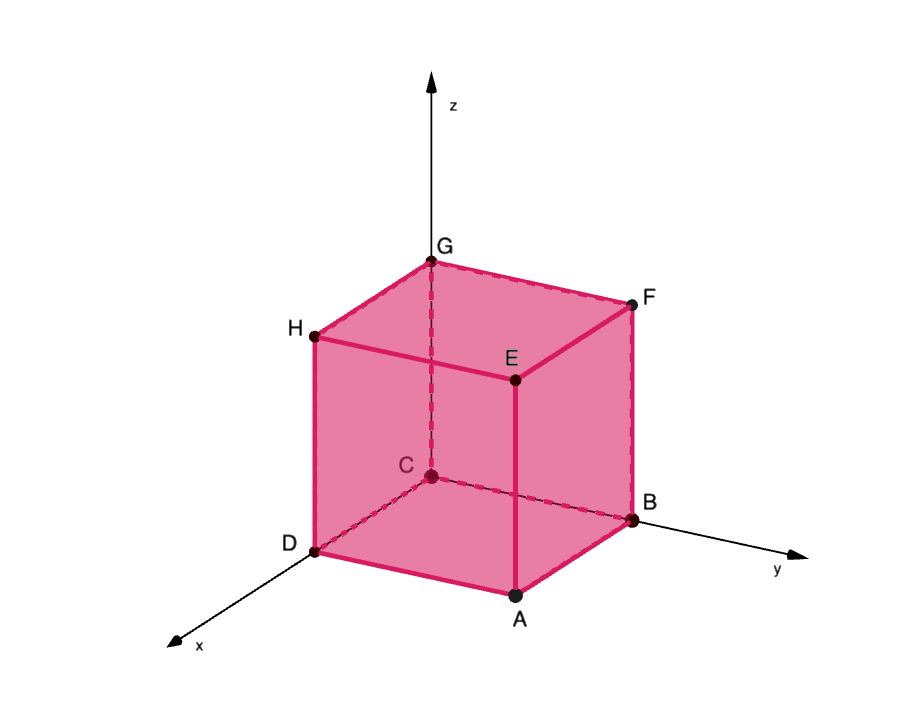
\includegraphics[width=0.7\textwidth, keepaspectratio]{images/einleitung/wuerfel_ortho_projektionen.png} 
    \caption{Regulärer Hexaeder $W$ mit Eckpunkten $A, B, \dots, H$.}
    \label{fig:einheitswürfel}
\end{figure}

Wir untersuchen, ob es eine invariante Eigenschaft in Bezug auf die projizierten Kantenlängen gibt. Eine Hypothese könnte lauten, dass die Summe der Längen aller projizierten Kanten eines Würfels bei einer Orthogonalprojektion unabhängig von der Lage der Projektionsebene ist. Um die Plausibilität dieser Hypothese zu prüfen, betrachten wir zunächst die Projektionen der Würfelkanten auf zwei verschiedene Ebenen. Sollte die Eigenschaft bereits für diese zwei Fälle nicht gelten, liesse sich die Hypothese direkt widerlegen. Das Nachvollziehen von Hypothesen an konkreten Instanzen ist zudem oftmals hilfreich, um ein besseres Verständnis aufzubauen und möglicherweise eine bessere Hypothese zu finden. Dieser Untersuchung gehen wir in Beispiel \ref{ex:wuerfelprojektionen} nach.



\begin{example}[Orthogonalprojektionen der Kanten eines Würfels auf eine Ebene] \label{ex:wuerfelprojektionen} 
Seien $E_1, E_2 \subset \mathbb{R}^3$ zwei Ebenen gegeben durch 

\begin{align}
    E_1:\ &x+y+z = 0,  \label{eq:ebene1}\\
    E_2:\ &x-y = 0 . \label{eq:ebene2}
\end{align}

 Sei $K_W$ die Menge der Kanten eines Würfels $W$, welcher in Abbildung \ref{fig:einheitswürfel} dargestellt ist. Wir wollen überprüfen, ob die Summe der Kantenlängen von einer Orthogonalprojektion auf diese beiden Ebenen identisch ist. Diese Behauptung kann wie folgt formuliert werden
\begin{align} \label{eq:hypothese1}
    \sum_{k \in K_W} \|\Pi_{E_1}(\vec{v}_k)\| = \sum_{k \in K_W} \|\Pi_{E_2}(\vec{v}_{k})\|,
\end{align}

wo $\Pi_{E_i}: \mathbb{R}^3 \rightarrow E_i$ die Orthogonalprojektion auf die Ebene $E_i \subset \mathbb{R}^3$ ist und $\vec{v}_k$ der zur Kante $k$ gehörende Richtungsvektor. Um diese Behauptung zu überprüfen, berechnen wir explizit die projizierten Kantenlängen eines regulären Hexaeders mit Kantenlänge $1$ und addieren diese auf. Diese Normierung vereinfacht die Rechnung, ohne die Allgemeingültigkeit einzuschränken, da die Ergebnisse für eine beliebige Kantenlänge $a$ lediglich um den Faktor $a$ skaliert würden. Die Ebene $E_1$, auf die wir projizieren, ist gegeben durch die Gleichung \eqref{eq:ebene1} mit dem Einheitsnormalenvektor 
\begin{align}
    \vec{n}_{E_1}  = \frac{1}{\sqrt{3}}\begin{pmatrix} 1 \\ 1 \\ 1 \end{pmatrix} .\nonumber
\end{align}

    \begin{figure}[htp]
    \centering
    \includegraphics[width=10cm]{images/einleitung/WürfelE1.png}
    \caption{Projektion der Kanten des Würfels auf die Ebene $E_1$ mit Normalenvektor $\vec{n}_{E_1}$.}
    \label{fig:würfelE1}
    \end{figure}

Bevor wir die Orthogonalprojektionen explizit berechnen, halten wir folgende Beobachtungen fest (siehe Abbildung \ref{fig:beobachtungenOrthogonalprojektionWurfel}):
\begin{itemize}
    \item Die Translation einer Strecke verändert die Länge ihrer Orthogonalprojektion auf eine Ebene nicht.
    \item Infolgedessen können wir jede Kante des Würfels als einen Vektor betrachten, indem wir ihren Fusspunkt in den Ursprung verschieben. 
\end{itemize}

    \begin{figure}[htp]
        \centering
        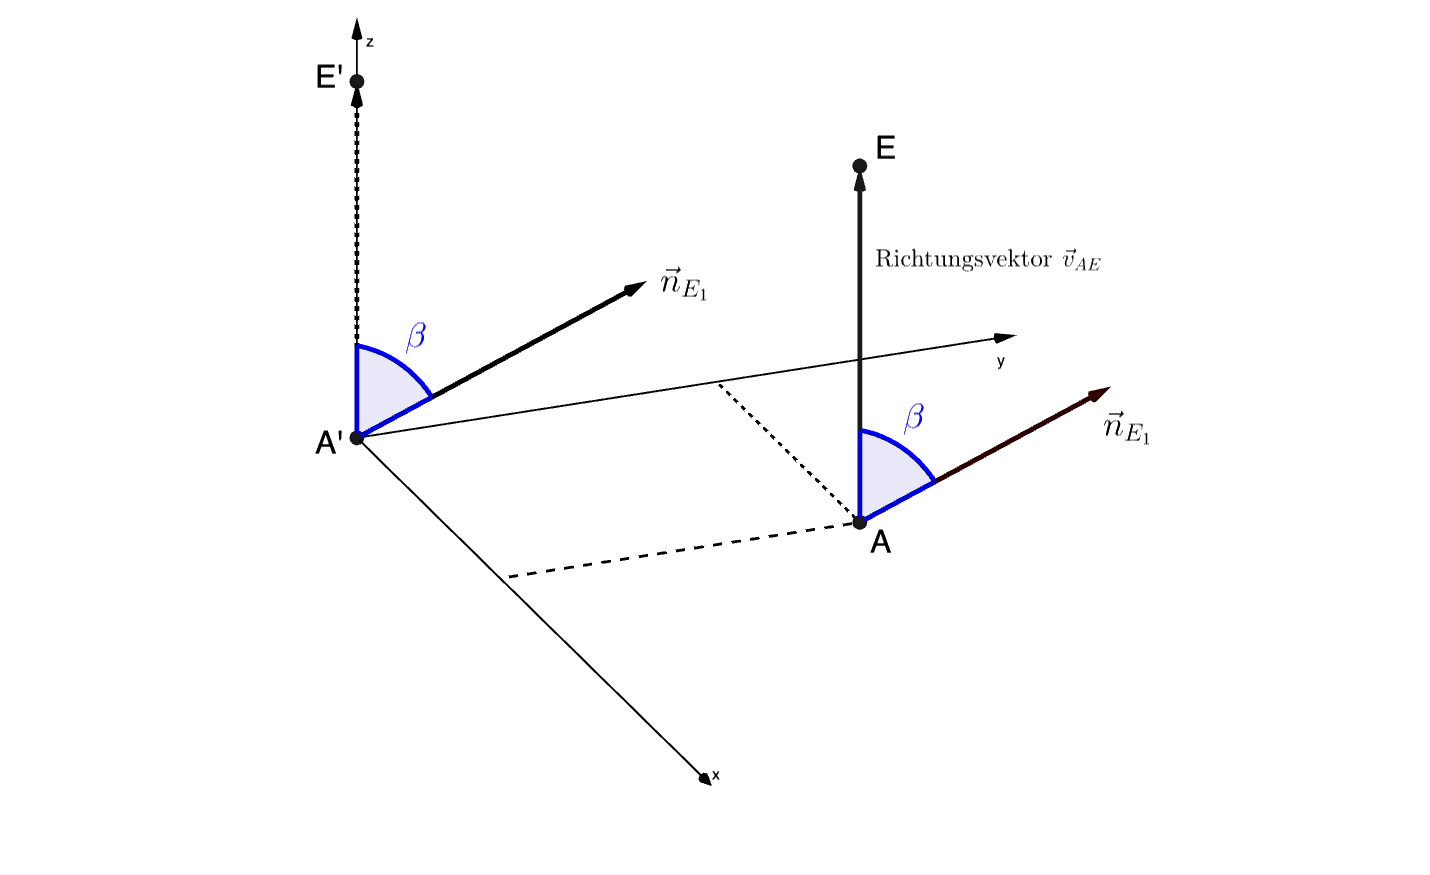
\includegraphics[width=10cm]{images/einleitung/VerschiebungKoordinatensystem.png}
        \caption{Beispiel der Translation des Richtungsvektors $\vec{v}_{AE}$. Der Winkel $\beta$ zum Normalenvektor $\vec{n}_{E_1}$ bleibt dabei erhalten.}
        \label{fig:beobachtungenOrthogonalprojektionWurfel}
    \end{figure}

Es lässt sich beobachten, dass die Strecken $\overline{CG}$, $\overline{CB}$ und $\overline{CD}$ den gleichen Winkel $\alpha$ mit dem Normalenvektor $\vec{n}_{E_1}$ einschliessen. Da alle Kanten des regulären Hexaeders zudem dieselbe Länge besitzen, sind auch ihre Projektionslängen identisch. Aus den vorangegangenen Überlegungen folgt, dass sämtliche Kanten des Würfels die gleiche Projektionslänge auf die Ebene $E_1$ aufweisen. Zur Berechnung dieser Länge können wir elementare trigonometrische Funktionen verwenden:

\begin{align} \label{eq:einführungsbeispielprojectionsimple}
    \|\Pi_{E_1}(\vec{v}_{CG})\| = \sin(\alpha) \cdot \|\vec{v}_{CG}\|,
\end{align}

wobei $\vec{v}_{CG}$ den Vektor der Kante $\overline{CG}$ repräsentiert und $\alpha$ der Winkel zwischen diesem Vektor und dem Normalenvektor $\vec{n}_{E_1}$ ist. Mit 
    \begin{align}
        \overline{CG}: \vec{v}_{CG}&=\begin{pmatrix} 0 \\ 0 \\ 1 \end{pmatrix},\|\vec{v}_{CG}\| = 1 \nonumber
    \end{align} sowie der Berechnungen
    \begin{align}
        \cos(\alpha) &= \frac{\vec{v}_{CG} \cdot \vec{n}_{E_1}}{\|\vec{v}_{CG}\| \|\vec{n}_{E_1}\|} = \frac{1}{\sqrt{3}} \nonumber \\
        \sin(\alpha) &= \sqrt{1-\cos^2(\alpha)} = \sqrt{\frac{2}{3}}, \nonumber
    \end{align}
    folgt aus Gleichung \eqref{eq:einführungsbeispielprojectionsimple}
    \begin{align}
        \|\Pi_{E_1}(\vec{v}_{CG})\| = \sqrt{\frac{2}{3}} \cdot 1= \sqrt{\frac{2}{3}} . \nonumber
    \end{align}
    Um die Summe aus Gleichung \eqref{eq:hypothese1} zu erhalten, müssen wir über alle Kanten in $K_W$ summieren und erhalten 
    \begin{align} \label{eq:summeebene1}
        \sum_{k \in K_W} \|\Pi_{E_1}(\vec{v}_{k})\| = 12 \cdot \sqrt{\frac{2}{3}} = 4\sqrt{6}.
    \end{align}
    
Wir behalten dieses Ergebnis im Hinterkopf und betrachten nun die Orthogonalprojektion auf die Ebene $E_2$ mit dem Einheitsnormalenvektor
    \begin{align}
        \vec{n}_{E_2} = \frac{1}{\sqrt{2}}\begin{pmatrix} 1 \\ -1 \\ 0 \end{pmatrix} .\nonumber
    \end{align}
    
    
    \begin{figure}[htp]
    \centering
    \includegraphics[width=0.7\textwidth, keepaspectratio]{images/einleitung/WürfelE2.png}
    \caption{Projektion der Kanten des Würfels auf die Ebene $E_2$ mit Normalenvektor $\vec{n}_{E_2}$.}
    \label{fig:würfelE2}
    \end{figure}
    
Aufgrund der Symmetrie des regulären Hexaeders können wir bei dieser Projektion zwei verschiedene Gruppen von Kanten unterscheiden:
\begin{itemize}
    \item Vier Kanten liegen parallel zur Ebene $E_2$ bzw. stehen orthogonal auf dem Normalenvektor $\vec{n}_{E_2}$, wie beispielsweise die Kante $\overline{CG}$.
    \item Die restlichen acht Kanten schliessen alle denselben Winkel $\alpha$, siehe Abbildung \ref{fig:würfelE2},mit dem Normalenvektor $\vec{n}_{E_2}$ ein, wie beispielsweise die Kante $\overline{GH}$.
\end{itemize}

Für die parallel zur Ebene $E_2$ verlaufenden Kanten gilt, dass ihre Länge bei der Projektion erhalten bleibt: 
\begin{align}
    \|\Pi_{E_2}(\vec{v}_{CG})\| = 1. \nonumber
\end{align}
    Für die anderen acht Kanten berechnen wir die Projektionslänge analog zu Gleichung \eqref{eq:einführungsbeispielprojectionsimple}. Da der Richtungsvektor $\vec{v}_{GH} = (1, 0, 0)^T$ einen Winkel von $\alpha = 45^\circ$ mit dem Normalenvektor $\vec{n}_{E_2}$ einschliesst, erhalten wir
\begin{align}
     \|\Pi_{E_2}(\vec{v}_{GH})\| = \sin\left(\frac{\pi}{4}\right) \cdot \|\vec{v}_{GH}\| = \frac{\sqrt{2}}{2} \cdot 1 = \frac{\sqrt{2}}{2}. \nonumber
\end{align}

Die Summation über alle 12 Kanten des regulären Hexaeders $W$ ergibt somit
\begin{align} \label{eq:summeebene2}
    \sum_{k \in K_W} \|\Pi_{E_2}(\vec{v}_k)\| = 4 \cdot 1 + 8 \cdot \frac{\sqrt{2}}{2} = 4 + 4\sqrt{2} = 4(1+\sqrt{2}).
\end{align}
Ein Vergleich der Ergebnisse aus den Gleichungen \eqref{eq:summeebene1} und \eqref{eq:summeebene2} zeigt deutlich, dass die Summen nicht übereinstimmen. Folglich ist die Summe der projizierten Kantenlängen unter einer Orthogonalprojektion nicht unabhängig von der Ebene. Die ursprüngliche Hypothese ist damit widerlegt. Dies beendet unser Beispiel.    
\end{example}


Wie wir in Beispiel \ref{ex:wuerfelprojektionen} gesehen haben, ist die Summe der projizierten Kantenlängen einer Orthogonalprojektion nicht unabhängig von der Projektionsebene. Eine invariante Eigenschaft unter Orthogonalprojektionen zu finden, scheint daher nicht trivial zu sein. Betrachten wir jedoch die Ergebnisse aus den Gleichungen \eqref{eq:summeebene1} und \eqref{eq:summeebene2} erneut, fällt bei genauerem Hinsehen auf, dass die Werte sehr nah beieinander liegen. Bei weiterer Untersuchung zeigt sich eine interessante Gesetzmässigkeit: Verwendet man die Quadrate der projizierten Kantenlängen scheinen die Summen tatsächlich identisch zu sein.

\begin{example} [Würfelprojektionen revisited] \label{ex:wuerfelprojektionen_revisited}
Wir passen unsere Hypothese an und betrachten die Summe der quadrierten Längen, d.h.
\begin{align}
    \sum_{k \in K_W} \|\Pi_{E_1}(\vec{v}_k)\|^2 = \sum_{k \in K_W} \|\Pi_{E_2}(\vec{v}_k)\|^2. \nonumber
\end{align}

Analog zu Beispiel \ref{ex:wuerfelprojektionen} berechnen wir die quadrierten Projektionslängen. Für die Ebene $E_1$ erhalten wir 
\begin{align}
    \sum_{k \in K_W} \|\Pi_{E_1}(\vec{v}_k)\|^2 = 12 \cdot \left(\sqrt{\frac{2}{3}}\right)^2 = 12 \cdot \frac{2}{3} = 8, \nonumber
\end{align}
und für die Ebene $E_2$
\begin{align}
    \sum_{k \in K_W} \|\Pi_{E_2}(\vec{v}_k)\|^2 = 4 \cdot 1^2 + 8 \cdot \left(\frac{\sqrt{2}}{2}\right)^2 = 4 + 8 \cdot \frac{1}{2} = 8. \nonumber
\end{align}
Dies bestätigt die angepasste Hypothese für diese beiden Fälle. Dies beendet unser Beispiel.
\end{example}

In Beispiel \ref{ex:wuerfelprojektionen_revisited} haben wir gesehen, dass unsere Vermutung für die Ebenen $E_1$ und $E_2$ zutrifft. Wie sich im Folgenden zeigen wird, ist dies kein Zufall. Diese Invarianz gilt nicht nur für das reguläre Hexaeder, sondern allgemein für alle Polyeder im $\mathbb{R}^3$, die gewisse Symmetriebedingungen erfüllen.

\subsubsection{Aufgaben}
\begin{exercise} \label{ex:verificationeinstiegesbeispielEbene3}
    Verifizieren Sie das Resultat aus Beispiel \ref{ex:wuerfelprojektionen_revisited} für die Ebene 
    \begin{align}
        E_3:\ x = 0. \nonumber
    \end{align}
    Berechnen Sie hierzu die Summe der quadrierten Längen der orthogonal projizierten Kanten des regulären Hexaeders mit Kantenlänge $1$ auf $E_3$.
\end{exercise}

\begin{exercise} \label{ex:geradesprisma}
    Betrachten Sie ein gerades Prisma mit einer quadratischen Grundfläche der Seitenlänge $a$ und der Höhe $h$, wobei $a \neq h$. Geben Sie zwei Projektionsebenen an und zeigen Sie durch Berechnung der jeweiligen Orthogonalprojektionen, dass die in Beispiel \ref{ex:wuerfelprojektionen_revisited} beschriebene Invarianz der quadrierten Kantenlängensumme für diesen Körper im Allgemeinen nicht gilt.
\end{exercise}